\documentclass[12pt,journal,compsoc]{IEEEtran}
\usepackage{listings}
\usepackage{cite}
\usepackage{graphicx}
\usepackage{float}
\usepackage[cmex10]{amsmath}
\usepackage{amsthm}
\usepackage{amsmath}
\usepackage{algorithm}
\usepackage{algorithmic}
\usepackage{url}

\theoremstyle{plain}% default
\newtheorem{thm}{Theorem}[section]
\newtheorem{lem}[thm]{Lemma}
\newtheorem{prop}[thm]{Proposition}
\newtheorem*{cor}{Corollary}
\newtheorem*{KL}{Klein’s Lemma}
\theoremstyle{definition}
\newtheorem{defn}{Definition}[section]
\newtheorem{conj}{Conjecture}[section]
\newtheorem{exmp}{Example}[section]
\theoremstyle{remark}
\newtheorem*{rem}{Remark}
\newtheorem*{note}{Note}
\newtheorem{case}{Case}

\begin{document}

\title{Proving Correctness with Finite Automata}
\author{Jeremy Wright}
\markboth{CSE 355 Extra Credit Project with JFLAP Integration}
{Shell \MakeLowercase{\textit{et al.}}: Bare Demo of IEEEtran.cls for Computer Society Journals}

\IEEEcompsoctitleabstractindextext{%
\begin{abstract}
%\boldmath
Finite Automata recognize the class of regular languages. This class is the most restrictive class from the Chomsky Hierarchy.
The beauty of this class is its simplicity. A simplicity that allows us to prove 
correctness of a program against its specification.  This isn't exhaustive
testing, rather we apply mathematical models from automata theory to prove with
certainty that a program meets its specification. Furthermore, by levering
properties of finite automata, if the unit under test (UUT) does not meet the
specification, our product can produce a test case demonstrating the failure.
\end{abstract}

\begin{IEEEkeywords}
Deterministic Finite State Machine, Nondeterministic, Model Based Design
\end{IEEEkeywords}}
\maketitle


\IEEEdisplaynotcompsoctitleabstractindextext

\IEEEpeerreviewmaketitle

\section{DFA Computational Model}
\IEEEPARstart{W}{ithin} computer-science we use mathematical objects to
describes computation. We can use mathematics to manipulate these computational
models in a rigorous and meaningful way. There are a series of models available
but the simplest of these allow us to prove more powerful properties. Discrete
Finite Automata is the simplest model as defined by within the Chomsky Hierarchy
\cite{wiki-chomsky}.  

\begin{defn}
    A language is called a \emph{regular language} if some finite automaton
    recognizes it.
    \label{def:regular}
\end{defn}

Discrete Finite Automata (DFA), generate the class of \emph{regular languages}.  
The class of regular languages has a powerful property, one can prove equivalence
of 2 models. While this seems like a straightforward thing to do, more powerful
computation models such as CFGs \cite[p.~172]{Sipser} and TM
\cite[p.192]{Sipser} do not have such a property. This is
something unique to Finite Automata alone. Using this one can define a machine
that accepts 2 DFAs as in Equation \ref{eq:dfa}. From Sipser, we know that
Equation \ref{eq:dfa} is decidable \cite[p.~169]{Sipser}.
\begin{multline}
    EQ_{DFA} = \left\{ \langle A, B \rangle  \mid  L( A ) = L( B ) \right\} \\
    \text{Where A and B are DFAs}
    \label{eq:dfa}
\end{multline}

\hfill \today


\section{Project}
Our goal is to build a system that can accept two ``programs'', one
a specification defining the correctness of the system. The second, an
implementation. Since the system leverages a property of regular languages the
problem must be simple enough to to express as a regular language i.e. the
problem must be expressible as a regular expression. Regular Languages are not extremely powerful, however  some very useful tools,
such as grep, leverage Regular Languages through their string representation
\emph{regular expressions}. 

Another useful property of regular
languages is, regular languages are closed under the standard set operations: union,
intersection, complement \cite[p.~45]{Sipser}.  We are now free to manipulate
our problem with standard set theory operations, and know we remain within the
context of regular languages \cite[p.~60]{Sipser}.

Our system will consume 2 programs, to determine if the
specification matches an implementation.
Equation \ref{eq:basis} defines how we intend to accomplish this. 
\begin{equation}
L( M ) = L( A ) \cap \overline{L ( S ) } 
\label{eq:basis}
\end{equation}
Equation \ref{eq:basis} follows that if a string exists in L(M) then there must
be a path in the model and the complement of the specification, ergo something
outside the specification. This is a bad path. After applying Equation
\ref{eq:basis}, we simply analyse L(M) to determine if our implementation matches
our specification.

Intuitively this makes sense.  If a program has ``bugs'' then the language the
implementation describes is not fully contained by the specification.  Our Model checker simply
needs to accept 2 DFAs, and apply Equation \ref{eq:basis}.  If the result is an
empty language as in we know that the implementation is contained by the specification.

\section{Model-Checker in C++}
The first step toward realizing an our verifier is to encode the mathematical
models into a representation which can be manipulated by the computer. 
Once we have a representable model, we can implement the required operations.
Firstly we have to convert the NFA representation to a DFA, then apply Equation
\ref{eq:basis}. Lastly, we run a search algorithm over the resultant DFA to
determine if the language is empty.

\subsection{DFA Representation}
The STL (Standard Template Library), offers 3 data structures which are
pertinent to representing the DFA: set, map, and multimap. The map made an
excellent tool to translate between states over a transition label.  
\begin{figure*}
    \begin{center}
        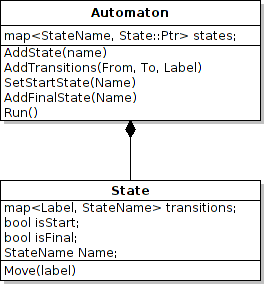
\includegraphics[width=2.5in]{UML.png}
        \label{fig:model}
        \caption{High-Level description of the Automaton Model.}
    \end{center}
\end{figure*}
The top level structure as in Figure 1, maps between a state name
and the state object.  Within the State, a second map translates a label to the
destination state name. One can repeat this process to traverse the entire
structure.

\subsection{Parallel Simulation of 2 DFAs}
Intersecting 2 DFAs amounts to simulating both DFAs in parallel and mapping the
destination. Algorithm \ref{alg:dfa_intersect} describes this operation. Prior
to the we build a list of all the states from each DFA. Then we run Algorithm
\ref{alg:dfa_intersect} which simulates both DFAs simultaneously. Finally it
adds a new transitions to the resulting DFA. 
\begin{algorithm}
    \caption{DFA Intersect}
    \label{alg:dfa_intersect}
\begin{algorithmic}
    \FORALL{$label \in alphabet$}
        \FORALL{$state \in combinedStates$}
            \STATE $ldest \gets M1.Dest(label)$
            \STATE $rdest \gets M2.Dest(label)$
            \STATE $FromState \gets pair<state1,state2>$
            \STATE $ToState \gets pair<ldest,rdest>$
            \STATE $DFA \gets new Transition(FromState, ToState, label)$
        \ENDFOR
    \ENDFOR
\end{algorithmic}
\end{algorithm}
This algorithm completes in $O(states * labels) < O(n^2)$. The inner loop traverses the states in
$O(n)$ time.  While the outer loop traverses all members of the alphabet, also
in linear time. 

\subsection{Finding an Accepted Path}
\begin{algorithm}
    \caption{FindPath(state, result)}
    \label{alg:FindPath}
\begin{algorithmic}
    \IF{Been Here Already}
        \RETURN false
    \ENDIF

    \IF{Is Accepting State}
        \RETURN true
    \ENDIF

    \FORALL{$state \gets AdjacentStates$}
        \IF{FindPath($state$, result)}
            \RETURN true
        \ENDIF
    \ENDFOR
    \STATE result.pop\_back()
    \RETURN false
\end{algorithmic}
\end{algorithm}
Finding an accepting path on the DFA is a classic case of a DFS search.
Essentially we traverse each branch of computation, recording where we've been.
If we reach a dead end, we recursively back up until there is another option.
Algorithm \ref{alg:FindPath}  describes this search process. 

Algorithm \ref{alg:FindPath} completes in $O(states+labes)$ time \cite{clr}


\subsection{Complement}
\begin{algorithm}
    \caption{DFA Complement}
    \label{alg:complement}
\begin{algorithmic}
    \FORALL{$state \in DFA$}
    \IF{$state = Accepting$}
            \STATE $state.final \gets false$
        \ELSE
            \STATE $state.final \gets true$
        \ENDIF
    \ENDFOR
\end{algorithmic}
\end{algorithm}

Finding the complement of the automaton is the easiest algorithm in this
application. Essentially just swap all the final and accept states. Algorithm
\ref{alg:complement} describes this succinctly. This algorithm completes in
linear time with the number of states $O(states)$.

\bibliographystyle{IEEEtran}
\bibliography{IEEEabrv,WrightSources}

\end{document}

